\chapter{图、表、公式示例}
图:包括曲线图、示意图、流程图、框图等。图序号一律用阿拉伯数字分章依序编码,如:图1.3、图2.11。
\par
每一个图应有简短确切的图名,连同图序号置于图的正下方。图名称、图中的内容字号为五号,中文字体为宋体,英文字体为Times New Roman,行距一般为单倍行距。图中坐标上标注的符号和缩略词必须与正文保持一致。引用图应在图题右上角标出文献来源;曲线图的纵横坐标必须标注“量、标准规定符号、单位”,这三者只有在不必要标明(如无量纲等)的情况下方可省略。
\par
图与正文之间一般应空一行。
\begin{figure}
\centering
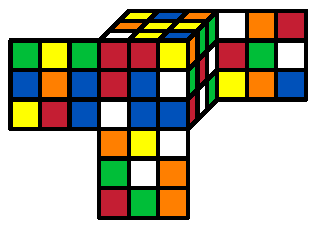
\includegraphics[width=5cm]{fig}\\
\caption{插图示例}
\end{figure}
\par
公式:正文中的公式、算式、方程式等必须编排序号,序号一律用阿拉伯数字分章依序编码,如:(3-32)、 (6-21)。
\par
对于较长的公式,另起行居中横排,只可在符号处(如:+、-、*、/、$<$$>$等)转行。公式序号标注于该式所在行(当有续行时,应标注于最后一行)的最右边。连续性的公式在“=”处排列整齐。大于999的整数或多于三位的小数,一律用半个阿拉伯数字符的小间隔分开;小于1的数应将0置于小数点之前。公式的行距一般为单倍行距。
\par
公式与正文之间一般应空一行。
\begin{equation}
\begin{split}
{X_{e1}}\left( {s,{n_1},{k_1}} \right) &= \left( {\begin{array}{*{20}{c}}
{{k_1}}\\
s
\end{array}} \right)\frac{{{n_1}!}}{{\left( {{n_1} - s} \right)!}}\sum\nolimits_{v = 0}^{\min \left( {{n_1} - s,{k_1} - s} \right)} {{{\left( { - 1} \right)}^v}\left( {\begin{array}{*{20}{c}}
{{k_1} - s}\\
v
\end{array}} \right)} \\
& \times \frac{{\left( {{n_1} - s} \right)!}}{{\left( {{n_1} - s - v} \right)!}}{\left( {{n_1} - s - v} \right)^{{k_1} - s - v}}
\end{split}
\end{equation}
\par
表:包括分类项目和数据,一般要求分类项目由左至右横排,数据从上到下竖列。
\par
分类项目横排中必须标明符号或单位,竖列的数据栏中不要出现“同上”、“同左”等词语,一律要填写具体的数字或文字。表序号一律用阿拉伯数字分章依序编码,如:表2.5、表10.3。
\par
每一个表格应有简短确切的题名,连同表序号置于表的正上方。表名称、表中的内容居中排列,字号为五号,中文字体为宋体,英文字体为Times New Roman,行距一般与正文保持一致。表格线统一用单线条,磅值为0.5磅。
\par
表格与正文之间一般应空一行。
\begin{table}
\renewcommand{\arraystretch}{1.5}
\caption{表格示例}
\label{tab0}
\centering
\begin{tabular}{|c|c|c|c|c|c|c|}
\hline
\multirow{2}{*}{\backslashbox{电性能参数}{馈电方式}}&\multirow{2}{*}{探针} & \multirow{2}{*}{环形缝隙}  & \multicolumn{2}{c|}{探针和缝隙} & \multicolumn{2}{c|}{缝隙和CPW} \\
\cline{4-7} & & &  探针 & 缝隙 & 缝隙 & CPW \\
\hline
谐振频率 & 9.5 GHz & 8.8 GHz & 9.4 GHz & 9.8 GHz & 9.2 GHz&9.3 GHz\\
\hline
\makecell[c]{带宽 \\ $|S_{11}|$ $<$-10 dB)}& 7.3\% & 4.5\% & 6.9\% & 6.8\% & 4.9\% & 5.3\% \\
\hline
\makecell[c]{隔离度\\(带内最差)} & -16.5 dB & -17 dB & \multicolumn{2}{c|}{-31 dB} & \multicolumn{2}{c|}{-22 dB} \\
\hline
方向图 & 不对称 & 对称 & 不对称 & 对称 & 对称 & 对称 \\
\hline
交叉极化电平 & 高 & 低 & 高 & 低 & 低 &低 \\
\hline
\end{tabular}
\end{table}
\par
计量单位:学位论文中出现的计量单位一律采用国务院1984年2月27日发布的《中华人民共和国法定计量单位》标准。
